\documentclass[12pt, a4paper]{article}
\usepackage{caption}
\usepackage{graphicx}
\usepackage{listings}
\usepackage{siunitx}
\usepackage{hyperref}
\def\checkmark{\tikz\fill[scale=0.4](0,.35) -- (.25,0) -- (1,.7) -- (.25,.15) -- cycle;}
\usepackage{tikz-network}
\hypersetup{
    colorlinks,
    citecolor=black,
    filecolor=black,
    linkcolor=black,
    urlcolor=black
}
\usepackage{amsmath, amsfonts, amssymb, amsthm}
\renewcommand{\thesubsubsection}{\thesubsection.\alph{subsubsection}}
\title{Algorithms and datastructures\\Exercises}
\date{2022}
\author{Kristoffer Klokker}
\begin{document}
	\maketitle
	\clearpage
	\tableofcontents
	\clearpage
		\setcounter{section}{5}
		\section{Uge}
			\subsection{Indicate the following according to figure 1.}
				\begin{figure}[h!]
					\centering
					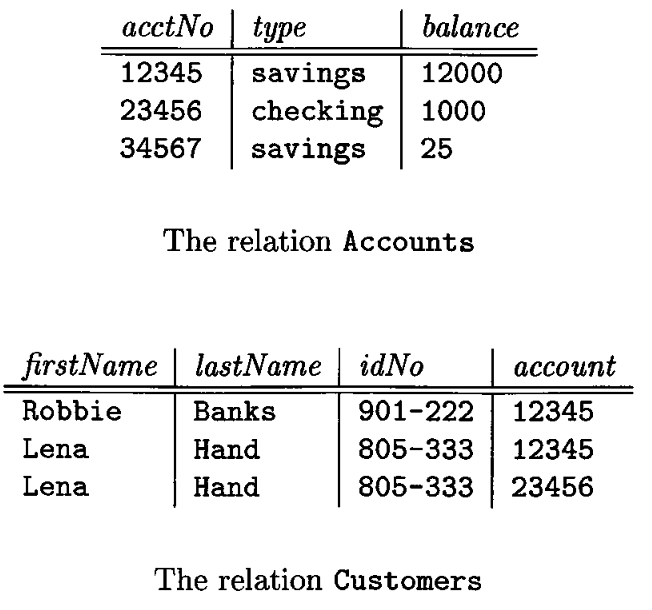
\includegraphics[width=300px]{assets/W6E1.png}
					\caption{Two relations of a banking database}
				\end{figure}
				\subsubsection{The attributes of each realtion}
					Accounts: $acctNo$, $type$, $balance$\\
					Customers: $firstName$, $lastName$, $idNo$, $account$
				\subsubsection{The tuples of each realtion}
					\begin{itemize}
						\item $12345, savings, 12000$
						\item $23456, checking, 1000$
						\item $34567, savings, 25$\\[5mm]
						\item $Robbie$, $Banks$, $901-222$, $12345$
						\item $Lena$, $Hand$, $805-333$, $12345$
						\item $Lena$, $Hand$, $805-333$, $23456$ 
					\end{itemize}
				\subsubsection{The components of one tuble of each realtion}
					$12000$\\
					$Banks$
				\subsubsection{The relation schema of each realtion}
					$Accounts(acctNo, type, balance)$\\
					$Customers(firstName, lastName, idNo,account)$
				\subsubsection{The database schema}
					$Accounts, Customers$
				\subsubsection{A suitable domain of each attribute}
					\begin{itemize}
						\item $acctNo$ - $INT$
						\item $type$ - $VARCHAR[20]$
						\item $balance$ - $INT$
						\item $firstName$ - $VARCHAR[20]$
						\item $lastName$ - $VARCHAR[20]$
						\item $idNo$ - $CHAR[7]$
						\item $account$ - $INT$
					\end{itemize}
				\subsubsection{Another equivalent way to present each relation.}
					The attributes could simply just be in a different order.
			\subsection{In a table with the following attributes which are valid example of keys}
				$$title, year, length, genre, studioName, producerC\#$$
				\begin{itemize}
					\item title, year
					\item title, year, studioName
					\item title, length
					\item length, genre, studioName, year
				\end{itemize}
			\subsection{How many ways can relation be represented if it has:}
				\subsubsection{Four attributes and five tuples}
					$4! \cdot 5! = 2880$\\
				\subsubsection{$n$ attributes and $m$ tuples}
					$n! \cdot m!$
			\subsection{Write a database schema of the following relations}
				The datasbase schema includes\\
				$Product(make, model, type)$\\
				$PC(model, speed,ram hd, price)$\\
				$Laptop(model, speed, ram, hd ,screen, price)$\\
				$Printer(model, color, type, price)$
				\subsubsection{Write a schema for $Product$}
					CREATE TABLE Product(VARCHAR[20] maker, INT model, INT type)\\
					The type is here an int where 0 is PC, 1 is laptop and 2 is printer. There is no foreign keys due to it being the lookup table for the other relations
				\subsubsection{Write a schema for $PC$}
					CREATE TABLE PC(INT model, FLOAT speed, INT ram, BOOLEAN hd, FLOAT prize, FOREIGN KEY(Products) REFERENCES Products(model))\\
					Here the model is a reference to products, speed is gigahertz of CPU
				\subsubsection{Write a schema for $Printer$}
					CREATE TABLE Printer(INT model, BOOLEAN color, VARCHAR[20] type, FLOAT price, FOREIGN KEY(Products) REFERENCES Products(model))\\
				\subsubsection{Write an alternation for Printer and delete the attribute color}
					ALTER TABKE Printer DROP color 
				\subsubsection{Add an $od$ attribute for PC, which defaults to none an otherwise can be cd or dvd}
					ALTER TABLE PC ADD VARCHAR[20] od DEFAULT 'none'
		\section{Uge}
			\subsection{Working with linear notation}
				The following exercises uses the following schema:\\
				$Product(maker, model, type)$\\
				$PC(model, speed,ram, hd, price)$\\
				$Laptop(model, speed, ram, hd ,screen, price)$\\
				$Printer(model, color, type, price)$
				\subsubsection{PC models which have speed of at least 3.00?}
					$\pi_{model}(\sigma_{speed > 3.00}(PC))$
				\subsubsection{PC manufacturers which makes PC with a hdd with at leat 100GB}
					$\pi_{maker}(Product \bowtie \sigma_{hd >= 100}(PC))$
				\subsubsection{Find model and price of all products made by manufacturer $B$}
					\begin{align*}
						man &:= \sigma_{maker = B}(Product)\\
						PCModelPrice &:= \pi_{model, price}(man \bowtie PC)\\
						LaptopModelPrice &:= \pi_{model, price}(man \bowtie Laptop)\\
						PrinterModelPrice &:= \pi_{model, price}(man \bowtie Printer)\\
						modPrice &:= PCModelPrice \cup LaptopModelPrice \cup PrinterModelPrice
					\end{align*}
				\subsubsection{Find model numbers of all color laster printers}
					$\pi_{model}(Product \bowtie \sigma_{color = 1 AND type = laser}(Printer))$
				\subsubsection{Find manufactures that sell Laptops but not PC}
					Due to algebra not including a method for group by I have answered in form of SQL queries.\\
					SELECT (SELECT maker FROM LAPTOP NATURAL JOIN Product GROUP BY maker)  -  (SELECT maker FROM PC NATURAL JOIN Product GROUP BY maker)
				\subsubsection{Find hd size which accour in two or more PC's}
					\begin{align*}
						PC = \pi_{model,hd}(PC)\\
						PC2(model2,hd) = \pi_{model,hd}(PC)\\
						hd = \pi_{hd}(\sigma_{model != model}(PC \bowtie PC2)
					\end{align*}
			\clearpage
			\subsection{In the following data, what is the result of $\pi_{speed}(PC)$ when treated as a bag and set}
				\begin{table}[h!]
				\begin{tabular}{|l|l|l|l|l|}
				\hline
				model & speed &ram &hd &price  \\\hline
				1001 &2.66 &1024 &250 &2114 \\\hline
				1002 &2.10 & 512 &250 &995   \\\hline
				1003 &1.42 & 512 & 80 &478      \\\hline
				1004 &2.80 &1024 &250 &649    \\\hline
				1005 &3.20 &512 &250 &630     \\\hline
				1006 &3.20 &1024 &320 &1049   \\\hline
				1007 &2.20 & 1024 &200 &510  \\\hline
				1008 &2.20 &2048 &250 &770  \\\hline
				1009 &2.00 &1024 &250 &650  \\\hline
				1010 &2.80 &2048 &300 &770    \\\hline
				1011 &1.86 &2048 &160 &959  \\\hline
				1012 &2.80 &1024 &160 &649    \\\hline
				1013 &3.06 &512 &80 &529     \\\hline
				\end{tabular}
				\end{table}
				\begin{minipage}[t]{0.5\textwidth}
				\begin{center}
				Bag\\
				\begin{tabular}{|l|}
				\hline
				speed\\\hline
				2.66 \\\hline
				2.10 \\\hline
				1.42 \\\hline
				2.80 \\\hline
				3.20 \\\hline
				3.20 \\\hline
				2.20 \\\hline
				2.20 \\\hline
				2.00 \\\hline
				2.80 \\\hline
				1.86 \\\hline
				2.80 \\\hline
				3.06 \\\hline
				\end{tabular}
				\end{center}
				\end{minipage}
				\begin{minipage}[t]{0.5\textwidth}
				\begin{center}
				Set\\
				\begin{tabular}{|l|}
				\hline
				speed\\\hline
				2.66 \\\hline
				2.10 \\\hline
				1.42 \\\hline
				2.80 \\\hline
				3.20 \\\hline
				2.20 \\\hline
				2.00 \\\hline
				2.80 \\\hline
				1.86 \\\hline
				3.06 \\\hline
				\end{tabular}
				\end{center}
				\end{minipage}
					
			
					
				
			
\end{document}


